\documentclass[a4paper, 14pt]{extarticle}

\usepackage[left=30mm, top=25mm, right=15mm, bottom=25mm]{geometry}
\linespread{1.3}
\pagenumbering{arabic}

\usepackage[backend=biber,
            language=auto, autolang=other, babel=other,
            citestyle=numeric-comp, bibstyle=gost-numeric,
            maxnames=3, sorting=none
            ]{biblatex}
\addbibresource{diploma.bib}   

\usepackage[T2A]{fontenc}
%\usepackage[russian, english]{babel} FUCK IT!
\usepackage[english,russian]{babel}
\usepackage[utf8]{inputenc}
% \usepackage[numbers]{natbib}
\usepackage{notoccite}
\usepackage{csquotes}
\usepackage{amsmath}
\usepackage{amsfonts}
\usepackage{amssymb}
\usepackage{graphicx}
\usepackage[percent]{overpic}
\usepackage{mathabx}
\usepackage{tabularx}
\usepackage{pifont}

\usepackage{pgfplots}
\pgfplotsset{width=10cm,compat=1.9}

\usepgfplotslibrary{external}
\tikzexternalize

\usepackage{unicode-math}
\usepackage{tikz, transparent, fancybox}
\usepackage[font=small,labelfont=bf]{caption}
\usetikzlibrary{trees}
\usetikzlibrary{positioning,decorations.pathreplacing,shapes}
\usepackage{smartdiagram}
\usetikzlibrary{arrows,automata}
\usetikzlibrary{positioning}
\usetikzlibrary{shapes,arrows}
\usetikzlibrary{calc, shapes, shadows, arrows, patterns}
\tikzstyle{line} = [ draw, -latex']  


%% pose estimation
%\theoremstyle{definition}
\newtheorem{example}{\inputencoding{utf8}Пример}

\newcommand{\RR}{{\mathbb{R}}}
\newcommand{\geqs}{\geqslant}
\newcommand{\leqs}{\leqslant}
\newcommand{\X}{{\mathcal X}}
\newcommand{\R}{{\mathcal R}}
\newcommand{\Iref}{I_\text{ref}}
\newcommand{\Iinc}{I_\text{inc}}
\newcommand{\vphi}{\varphi}
\newcommand{\ol}{\overline}
\newcommand{\norm}[1]{\left\|#1\right\|}
\newcommand\myeq{\mathrel{\stackrel{\makebox[0pt]{\mbox{\normalfont\tiny def}}}{=}}}
\newcommand{\relu}{\text{ReLU}}

            
            
            


\newcommand\suchthat[1][]{\;#1|\;}
%\newcommand\norm[1]{\left\|#1\right\|}
\newcommand\slfrac[2]{\left.#1\middle/#2\right.}
\DeclareMathOperator\rank{rank}
\newcommand{\ie}{{\inputencoding{utf8}т.\,е.}\xspace}
\newcommand{\te}{\ie}
\newcommand{\td}{{\inputencoding{utf8}т.\,д.}\xspace}
\newcommand{\tp}{{\inputencoding{utf8}т.\,п.}\xspace}
\newcommand{\dr}{{\inputencoding{utf8}др.}\xspace}
%\newcommand\RR{\mathbb{R}}
\newcommand\Rot{\mathfrak{R}}
\newcommand\rot{\mathfrak{r}}
\newcommand\vrglo{\vec r_\text{glo}}
\newcommand\vRglo{\vec R_\text{glo}}
\newcommand\viglo{\vec i_\text{glo}}
\newcommand\vjglo{\vec j_\text{glo}}
\newcommand\vkglo{\vec k_\text{glo}}
\newcommand\vIglo{\vec I_\text{glo}}
\newcommand\vJglo{\vec J_\text{glo}}
\newcommand\vKglo{\vec K_\text{glo}}
\newcommand\vrgnd{\vec r_\text{gnd}}
\newcommand\vRgnd{\vec R_\text{gnd}}
\newcommand\vignd{\vec i_\text{gnd}}
\newcommand\vjgnd{\vec j_\text{gnd}}
\newcommand\vkgnd{\vec k_\text{gnd}}
\newcommand\ignd[1][]{i_\text{gnd\ifthenelse{\equal{#1}{}}{}{\,}#1}}
\newcommand\jgnd[1][]{j_\text{gnd\ifthenelse{\equal{#1}{}}{}{\,}#1}}
\newcommand\kgnd[1][]{k_\text{gnd\ifthenelse{\equal{#1}{}}{}{\,}#1}}
\newcommand\vIgnd{\vec I_\text{gnd}}
\newcommand\vJgnd{\vec J_\text{gnd}}
\newcommand\vKgnd{\vec K_\text{gnd}}
\newcommand\Acam[1][]{A_{\text{cam}\ifthenelse{\equal{#1}{}}{}{\,}#1}}
\newcommand\Rotcam[1][]{\Rot_{\text{cam}\ifthenelse{\equal{#1}{}}{}{\,}#1}}
\newcommand\rotcam[1][]{\rot_{\text{cam}\ifthenelse{\equal{#1}{}}{}{\,}#1}}
\newcommand\vrcam[1][]{\vec r_{\text{cam}\ifthenelse{\equal{#1}{}}{}{\,}#1}}
\newcommand\vtcam[1][]{\vec t_{\text{cam}\ifthenelse{\equal{#1}{}}{}{\,}#1}}
\newcommand\Ecam{E_\text{cam}}
\newcommand\Eloc{E_\text{loc}}

% --- мои операции - Ященко Михаил 435 --- %
\newcommand\ptime{\ding{42}}
\newcommand{\pplus}{\oplus}
\newtheorem{theorem}{Теорема}
\newtheorem{axiom}{Аксиома}
\newtheorem{definition}{Определение}
\DeclareMathOperator{\supp}{supp}
% \renewcommand{\refname}{Bibliography}
\DeclareMathOperator*{\argmax}{arg\,max}
\DeclareMathOperator*{\argmin}{arg\,min}
%\DeclareUnicodeCharacter{0301}{*************************************}
%%
\begin{document}
\begin{titlepage}
\begin{center}



{\small ФЕДЕРАЛЬНОЕ ГОСУДАРСТВЕННОЕ БЮДЖЕТНОЕ ОБРАЗОВАТЕЛЬНОЕ 
УЧРЕЖДЕНИЕ ВЫСШЕГО ОБРАЗОВАНИЯ 

<<МОСКОВСКИЙ ГОСУДАРСТВЕННЫЙ УНИВЕРСИТЕТ

имени М.В. ЛОМОНОСОВА>>
\ \\[1ex]
ФИЗИЧЕСКИЙ ФАКУЛЬТЕТ МГУ }
\ \\[0.8ex]
Кафедра математического моделирования и информатики
\ \\[0.8ex] 
\hrule 

\vspace{1cm}

{\large ДИПЛОМНАЯ РАБОТА}

{\large\bf <<Мера специфичности качественных распределений возможностей>> \\}
\ \\[2ex]
\begin{flushright}
\begin{minipage}{0.42\textwidth}
{\bf Выполнил}  \\ студент 435 группы \\ Ященко~М.~А.
\vspace{8mm}
\vspace{1mm}
{\small }
\\[1ex]
{\bf Научный руководитель} \\ к.ф.-м.н. Зубюк~А.~В.

\vspace{30mm}

\end{minipage}
\end{flushright}
\end{center}
\hspace{3em}

\vfill
\begin{flushleft}
\begin{minipage}{0.4\textwidth}
{\bf Допущен к защите} \\ {\small Зав. кафедрой математического моделирования  и информатики\\\\
\underline{\hspace{6cm}}\\д.ф.-м.н. проф. Чуличков~А.~И.}
\vspace{8mm}
\vspace{1mm}
{\small }
\end{minipage}
\end{flushleft}

\vfill
\begin{center}
Москва
\vfill
2022
\end{center}

\end{titlepage}


\newpage
\setcounter{page}{2}

\tableofcontents

\newpage
\setcounter{page}{3}
\pagestyle{plain}
\section*{Введение}
Теория возможностей, разработанная Ю.П. Пытьевым, определяет возможность как монотонную меру $\Pi$, числовые значения которой лежат в [0,1]. Если $\Pi(A) = 0$, то A --- невозможно, если $\Pi(A) > \Pi(B)$ --- A более возможно чем B, если $\Pi(A) = \Pi(B)$, то A и B одинаково возможны. Все результаты, полученные с помощью теории возможностей Пытьева, инвариантны к любому строго возврастающему полунепрерывному снизу преобразованию всех значений возможностей с фиксированными точками 0 и 1. Этот факт позволяет присваивать числовые значения возможностям, используя индивидуальную субъективную шкалу значений возможностей. В отличие от теории возможностей Заде, основанной на нечетких множествах, где специфичность распределений возможностей оценивается посредством включения нечеткого множества, а распределение $\pi_1$ более специфично, чем $\pi_2$, если $\pi_1 \leqslant \pi_2$ поточечно, в теории возможностей Пытьева такой подход не может быть применен, если числовые значения $\pi_1$ и $\pi_2$ присваиваются в разных субъективных шкалах. 

На основе теории возможностей Пытьева в работе \cite{zubyuk-fss-2018} было введено отношение специфичности распределений возможностей. 
% Независимо от того, проводится ли исследование в рамках теории возможностей Пытьева, полученные результаты не ограничиваются ею и могут быть использованы в других вариантах теории возможностей. 

Затем в работе \cite{ag-op-2021} на основе отношения специфичности были введены агрегирующие операции --- супремум и инфимум. При принятии групповых решений эти операторы могут быть использованы для объединения распределний возможностей, представляющих мнения разных экспертов по одному и тому же вопросу, в новое распределение возможностей, которое представляет собой консенсус. Такое распределение дает решение, приемлимые всеми вовлеченными экспертами.

В рамках дипломной работы были поставлена цель --- разработать алгоритм, которые позволит находить расстояние в решетке на классах эквивалентностей. Для достижения данной цели необходимо выполнить следующие задачи:
\begin{itemize}
    % \item продвинуться в понимании теории возможностей,
    \item разработать алгоритм 
    \item сформулировать определение меры специфичности или меры согласованности на основе операций супремум и инфимум.
\end{itemize}

\section{Теория возможностей Пытьева как альтернатива теории вероятностей} 
\subsection{Теория возможностей в случае единичного испытания в случайном эксперименте} \label{11}
Пусть $\Omega$ --- множество элементарных исходов некоторого случайного эксперимента, ${\cal F}$ --- алгебра событий, и P: ${\cal F} \rightarrow [0, 1]$ - вероятность, определенная на ${\cal F}$. Тогда $(\Omega, {\cal F}, P)$ - вероятностное пространство этого эксперимента.

Согласно закону больших чисел относительная частота $\nu_n(A) = n_A/n$ любого события $A \in {\cal F}$ в серии n независимых одинаковых экспериментов близко к вероятности P(A), если n большое, $n_A$ --- число раз, когда событие случилось. Этот факт, являющийся эмпирической основой теории вероятностей, является единственным, что позволяет разумно интерпретировать числовые значения вероятностей. Однако, если эксперимент единственный (n = 1), то закон больших чисел не применим, и определенные значения вероятностей не имеют смысла. Тем не менее, даже если n = 1, ранжирование событий по их вероятностям может быть разумно интерпретировано: несмотря на то, что высокая вероятность события не гарантирует, что событие произойдет, а низкая вероятность не гарантирует обратного, естественно признать, что скорее произойдет более вероятное событие, чем менее вероятное.

Таким образом, мы пришли к выводу, что в случае единичного испытания числовые значения вероятностей ничего не значат, но ранжирование событий по их вероятностям разумно интерпретируемо.

Приняв этот вывод, следует рассмотреть возможность отказа от вероятностного подхода в случае единичного испытания. Действительно, выводы теории вероятностей, полученные с использованием вероятностного пространства $(\Omega, {\cal F}, P)$ в общем случае не инвариантны к изменению его на $(\Omega, {\cal F}, P')$, если вероятность $P'$ имеет другие численные значения, но при этом вероятности одинаково упорядочены. Математически это вытекает из того факта, что отображение диапазона вероятностей [0, 1] с сохранением порядка само по себе, как правило, не сохраняет обычное сложение “+” и умножение “×” действительных чисел, используемых в теории вероятностей для работы с числовыми значениями вероятностей.

\subsection{Теория возможностей как основа для получения инвариантных результатов}
Для решения проблемы, описанной выше, профессор Ю. П. Пытьев разработал новую ветвь теории возможностей. Он определил возможность $\Pi$ как функцию ${\cal F} \rightarrow [0, 1]$ такую, что $\Pi(\varnothing) = 0$ и $\Pi(\Omega) = 1$. В отличие от теории вероятностей теория возможностей Пытьева позволяет получать одни и те же результаты, используя любые две возможности $\Pi$ и $\Pi'$, удовлетворяющие следующим условиям для любых событий $A, B \in {\cal F}$:
\begin{itemize}
    \item $\Pi(A) = \Pi(B) \Leftrightarrow \Pi'(A) = \Pi'(B)$ --- события A и B равновозможны,
    \item $\Pi(A) < \Pi(B) \Leftrightarrow \Pi'(A) < \Pi'(B)$ --- событие A менее возможно, чем событие B.
\end{itemize}

\textbf{Принцип относительности в теории возможностей.} Возможности $\Pi$ и $\Pi'$ эквивалентны, если существует строго возрастающая непрерывная снизу функция $\gamma$: $\mathcal{L}_{\Pi} \rightarrow \mathcal{L}_{\Pi'}$, такая, что $\Pi'(A) = \gamma(\Pi(A))$ для любого $A \in {\cal F}$, $\gamma(0) = 0$, $\gamma(1) = 1$, 
где $\mathcal{L}_{\Pi} = \{ \Pi(A) | A \in {\cal F} \}, \mathcal{L}_{\Pi'} = \{ \Pi'(A) | A \in {\cal F} \}$.

Согласно принципу относительности, конкретная мера возможности полностью определяется бинарным отношением $\mathcal{R}$ на $\mathcal{F}$ и наоборот:
\begin{equation}
    \begin{gathered}
        \Pi(A) \leq \Pi(B) \Leftrightarrow (A, B) \in \mathcal{R},\\
        \Pi(A) < \Pi(B) \Leftrightarrow (A, B) \in \mathcal{R} и (B, A) \notin \mathcal{R},\\
        \Pi(A) = \Pi(B) \Leftrightarrow (A, B) \in \mathcal{R} и (B, A) \in \mathcal{R}.
    \end{gathered}
\end{equation}

\begin{figure}[h]
    	\begin{center}
	   % \raisebox{70pt}{\parbox{0.3\textwidth}{Three equivalent representations $\pi_1,\ \pi_2,\ \pi_3$ of the same comparative possibility distribution:}}
		\begin{tikzpicture}
			\begin{axis}[
			width = 0.5\textwidth, height = 0.37\textwidth,
			axis lines = middle,
			xlabel = {$\omega$}, ylabel = {$\pi(\omega) \stackrel{\Delta}{=} \Pi(\{\omega\})$},
			ymin = 0, ymax = 1.4,
			xmin = 0, xmax = 2.6,
			xtick = {0.2, 0.7, 1.2, 1.7, 2.2},
			xticklabels = {$\omega_1$, ,$\omega_2$, ,$\omega_3$},
			ytick = {0, 1}, extra y ticks = 0
			]
			\addplot[black, very thick, dotted] table[x=omega, y=p1] {pictures/equivalent_possibilities.txt};
			\addplot[black, very thick] table[x=omega, y=p2] {pictures/equivalent_possibilities.txt};
			\addplot[black, very thick, dashed] table[x=omega, y=p3] {pictures/equivalent_possibilities.txt};
			\end{axis}
		\end{tikzpicture}
		\caption{Три эквивалентные возможности представлены их распределениями — функциями, которые присваивают значение возможности каждому элементарному событию $\omega \in \Omega = (-\infty, \infty)$. Теория возможностей Пытьева дает одни и те же результаты (например, в задачах принятия решений) для всех этих возможностей.}
	\end{center}
\end{figure}

\subsection{Алгебраические операции над числовыми значениями возможностей}
Меры возможностей можно использовать для построения сравнительных соотношений возможностей на $\mathcal{F}$. Это может казаться удобным теоретически, однако соотношения на $\mathcal{F}$ вряд ли могут быть использованы на практике. Если $\Omega$ состоит из $n$ элементарных событий, то в алгебре $\mathcal{F}$ содержится $2^n$ событий. В таком случае полное отношение $\mathcal{R}$ определяет $2^n(2^n - 1)$ событий $(A, B) \in \mathcal{R}$ или $(A, B) \notin \mathcal{R}$, что на практике невозможно использовать, так как уже для $n = 20$, $2^n(2^n - 1) > 10^{12}$.

Чтобы обойти подобные ограничения Ю.П. Пытьев предложил использовать меры возможности с численными значениями в [0, 1], также как в теории вероятностей, где возможность любого события может быть посчитана, используя операции ``+'' (или ``$\int$'') и ``$\times$''. Однако эти операции не могут быть использованы, потому что они не дают инвариантных результатов, как того требует принцип относительности. Это делает определение правильных алгебраических операций на  области определения возможностей [0, 1] одним из главных аспектов теории возможностей Пытьева. Вводится \textbf{шкала значений возможностей} $\mathcal{L} = ([0, 1], \leq, \oplus, \ptime)$, которая представляет собой единичный интервал [0, 1] с определенным отношением порядка действительных чисел ``$\leq$'' и двумя алгебраическими операциями ``$\oplus$'' и ``$\ptime$'', ведущими себя как сложение и умножение. Тогда любая возможность --- это функция $\mathcal{F}\to\mathcal{L}$ вместо простого $\mathcal{F}\to[0, 1]$

В шкале $\mathcal{L}$ алгебраическим операциям были присвоены символы $\oplus$ и $\ptime$, но не были определены эти операции.


\begin{theorem} \label{t1}
(см. \cite{pyt2007possibility}) Если бинарные операции ``$\oplus$'' и ``$\ptime$'' осуществляют непрерывное отображение $[0, 1]\times[0,1]\rightarrow[0,1]$ и обладают свойствами $\gamma(a \oplus b) = \gamma(a) \oplus \gamma(b)$, $\gamma(a \ptime b) = \gamma(a) \ptime \gamma(b)$ для любой строго возрастающей полунепрерывной снизу функции $\gamma$ такой, что $\gamma(0) = 0$ и $\gamma(1) = 1$, и $0 \oplus a = a$, $0 \ptime a = 0$, $1 \oplus a = a$, $1 \ptime a = a$ для любого $a \in [0,1]$, тогда $a \oplus b = max\{a, b\}$, $a \ptime b = min\{a, b\}$, $a, b \in [0, 1]$.  
\end{theorem}

\subsection{Возможность, ее распределение, и пространство возможностей}
Обобщая вышеприведенные соображения, возможность $\Pi$ может быть определена, как функция $\mathcal{F}\to\mathcal{L}$, удовлетворяющая следующим аксиомам:
\begin{axiom}
 $\Pi(\varnothing) = 0,$
\end{axiom}
\begin{axiom}
$\Pi(\Omega) = 1,$
\end{axiom}
\begin{axiom}
\[
\Pi(\bigcup_{A\in\kappa} A) = \underset{A\in\kappa}\pplus \Pi(A) \quad \forall \kappa \subset \mathcal{F},
\]
где ``$\pplus$'' --- операция суммирования на $\mathcal{L}$: ``max'' для конечного $\kappa$, ``sup'' в противном случае.
\end{axiom}

Пространство возможностей --- это триплет $(\Omega, 2^{\Omega}, \Pi)$, рассматриваемый как модель ``нечеткого'' эксперимента. Любое подмножество $A \in 2^{\Omega}$ называется \textbf{событием}. Функция $\pi$: $\mathcal{F}\to\mathcal{L}$ определяемая, как
\begin{equation}
    \pi(\omega) = \Pi(\{\omega\}), \quad \omega \in \Omega,
\end{equation}
распределение возможности $\Pi$. Нормировка функции: $\pplus_{\omega\in\Omega} \pi(\omega) = sup_{\omega\in\Omega} \pi(\omega) = 1$. Возможность любого события $A \in 2^{\Omega}$ может быть вычислена как
\begin{equation}
    \Pi(A) = \underset{\omega \in A}\pplus \pi(\omega), \quad A \in 2^{\Omega}.
\end{equation}

Если $\pi$ --- распределение возможностей $\Pi$, множество $\mathcal{L}_{\Pi} = \{\Pi(A) | A \in 2^{\Omega}\}$ может быть выражено как
\begin{equation}
    \mathcal{L}_{\Pi} = \{\underset{\omega \in A}\pplus \pi(\omega) | A \in 2^{\Omega}, A \neq \varnothing\} \cup \{0\}.
\end{equation}

Принцип относительности может быть переформулирован в терминах распределений возможностей следующим образом:

\noindent\textbf{Принцип относительности в терминах распределений возможностей.} Возможности $\Pi$ и $\Pi'$ с распределениями $\pi$ и $\pi'$ эквивалентны, если существует строго возрастающая, полунепрерывная снизу функция $\gamma$: $\mathcal{L}_{\Pi} \to \mathcal{L}_{\Pi'}$, такая, что $\pi'(\omega) = \gamma(\pi(\omega))$ для любого $\omega \in \Omega$, $\gamma(0) = 0$, $\gamma(1) = 1$, где $\mathcal{L}_{\Pi} = \{\pplus_{\omega \in A} \pi(\omega) | A \in 2^{\Omega}, A \neq \varnothing\} \cup \{0\}$, $\mathcal{L}_{\Pi'} = \{\pplus_{\omega \in A} \pi'(\omega) | A \in 2^{\Omega}, A \neq \varnothing\} \cup \{0\}$.

\subsection{Возможность, как мера предпочтения в случайном эксперименте}
Как описано в \ref{11}, порядок предпочтений в алгебре событий $\mathcal{F}$ естественным образом связан с ранжированием событий по их вероятностям. Эта согласованность вероятности и возможности может быть представлена следующим математическим принципом: 

\noindent\textbf{Слабый принцип согласованности вероятности и возможности.} Возможность $\Pi$: $\mathcal{F}\to\mathcal{L}$ согласована с вероятностью P: $\mathcal{F}\to[0,1]$, если из $P(A) \leq P(B)$ следует $\Pi(A) \leq \Pi(B)$ для любых событий $A, B \in \mathcal{F}$.

Согласно этому принципу, строго более вероятное событие не может быть строго менее возможным, и наоборот. Однако некоторые события с разной вероятностью могут иметь одинаковые возможности. Пусть \textbf{1}:  $\textbf{1}(A) = 1$ для любого $A \in \mathcal{F}$, $A \neq \varnothing$ --- модель полного незнания, согласующаяся с любой веротяностью P. Тогда сформулированный выше принцип допускает возможность, что $\Pi$ --- абсолютно неинформативно и поэтому данный принцип называется слабым. Для решения этой проблемы можно сформулировать более строгий принцип:

\noindent\textbf{Сильный принцип согласованности вероятности и возможности.} Возможность $\Pi$: $\mathcal{F}\to\mathcal{L}$ максимально согласована с вероятностью P: $\mathcal{F}\to[0,1]$, если $\Pi$ согласована с P и из $\Pi(A) = \Pi(B)$ следует $\Pi'(A) = \Pi'(B)$ для любой другой возможности $\Pi'$ согласованной с P и для любых событий $A, B \in \mathcal{F}$.

Максимально согласованная возможность - это такая возможность из класса всех согласованных, которая отличает события лучше, чем любая другая возможность из этого класса, другими словами, это наиболее информативная согласованная возможность. Как показано в \cite{pyt2002stochastic}, максимально согласованная возможность уникальна с точностью до эквивалентности (определение эквивалентности вводится принципом относительности выше). Для $\Omega = {\omega_1, \omega_2, \ldots}$, максимально солгласованная возможность существует и определяется следующим образом:
\begin{equation}
    \pi_i > \pi_j \quad \text{если} \quad p_i > p_j \quad \text{и} \quad p_i > \sum_{k: p_i > p_k} p_k,
\end{equation}
\begin{equation}
    \pi_i \leq \pi_j \quad \text{в противном случае,}
\end{equation}
где $p_i = p(\omega_i)$, $\pi_i = \pi(\omega_i)$, $i = 1, 2, \ldots$ В случае абсолютно непрерывной вероятности максимально согласованная возможность существует и всегда тривиальна: $\pi(\omega) = 1$, $\forall \omega \in \Omega$.

Если $\Pi$ максимально согласована с P, пространство возможностей $(\Omega, 2^{\Omega}, \Pi)$ рассматривается, как возможностная модель случайного эксперимента со следующей вероятностной моделью: $(\Omega, \mathcal{F}, P)$.

Теория возможностей Пытьева имеет много общего со сравнительными вероятностными упорядоченностями. Сравнительная вероятность на $\mathcal{F}$ это частичное бинарное отношение $\mathcal{R}$ на $\mathcal{F}$: $A, B \in \mathcal{R}$ означает, что A не более вероятно, чем B. Теория возможностей Пытьева основана на аналогичной идее. Однако между этими теориями есть некоторые различия. Прежде всего, отношение $\mathcal{R}$ является частичным для сравнительной вероятности и является полным в теории возможностей Пытьева.

Однако главное отличие заключается в принятии решений. Чтобы сделать сравнительную вероятность пригодной для этой цели, отношение $\mathcal{R}$ представлено обычной вероятностной мерой P, которая совместима с $\mathcal{R}$ в следующем смысле: $(A, B) \in \mathcal{R} \Rightarrow P(A) \leq P(B)$. Затем проблемы принятия решений решаются с использованием совместимой вероятности P, а также обычных вероятностных методов принятия решений. Однако в некоторых случаях отношение $\mathcal{R}$ может быть представлено множеством вероятностей, которые приводят к различным решениям. Чтобы решить эту проблему, сравнительная теория вероятностей фокусируется на единственности представления $\mathcal{R}$ и исследует надежность принятия решений, если представление не является уникальным.

Теория возможностей Пытьева, напротив, полностью отвергает вероятностный подход и скорее фокусируется на разработке нового исчисления полных бинарных отношений на $\mathcal{F}$, чтобы иметь возможность принимать инвариантные решения. Результат приводиться в теореме \ref{t1}: для того, чтобы получить инвариантные решения, можно представить отношение $\mathcal{R}$ с помощью некоторой численной меры возможностей $\Pi$ совместимой с $\mathcal{R}$ (в следующем смысле: $(A, B) \in \mathcal{R} \Leftrightarrow \Pi(A) \leq \Pi(B)$) и затем пользоваться мерой $\Pi$ с помощью алгебраических операций ``$\pplus$'' (``max'') и ``$\ptime$'' (``min'').

Теория возможностей Пытьева не является единственной теорией, устанавливающей связи между вероятностями и возможностями. Приведенное выше преобразование вероятность-возможность согласуется с той точки зрения, что “распределения возможностей являются более слабыми представлениями неопределенности, чем распределение вероятностей”, и “переход от возможности к вероятности приводит к увеличению информативности рассматриваемого представления, в то время как обратный переход означает потерю информации”. В случае теории возможностей Пытьева этот факт можно рассматривать следующим образом: для возможности $\Pi$ существует множество различных вероятностей, таких, что $\Pi$ максимально согласуется с ними, класс всех таких вероятностей обозначается $\textbf{P}(\Pi)$, в то время как для любой вероятности P существует единственная (до эквивалентности) возможность $\Pi$, максимально совместимая с P.

Числовые значения меры возможности, кроме 0 и 1, не имеют смысла в теории Пытьева, поэтому преобразования вероятность–возможность и возможность–вероятность не могут быть выражены прямыми формулами, такими как
\begin{equation}
    p_i = \sum_{j = i}^n (\pi_j - \pi_{j+1}) / j, \quad \pi_i = \sum_{j = i}^n \pi_j
\end{equation}
также как в других теориях. Вместо этого они выражаются линейными условиями (системой линейных уравнений и неравенств), такими как \cite{dubois1980fuzzy}.

\subsection{Нечеткий элемент}
Понятие нечеткого элемента в теории возможностей Пытьева аналогично понятию случайная величина в теории вероятностей \cite{pytyev-poss_in_patrec-iii}. 
\begin{definition}
\label{101}
Нечеткий элемент $\xi$ со значениями в X --- функция $\xi$: $\Omega \to X$.
\end{definition}

Сравним с определением случайной величины:
\begin{definition}
\label{102}
Случайная величина $\xi$ --- функция $\xi$: $\Omega \to (-\infty, \infty)$, такая что $\{\omega: \xi(\omega) < x \} \in \mathcal{F}$ для любого $x \in (- \infty, \infty)$.
\end{definition}

Условие $\{\omega: \xi(\omega) < x \} \in \mathcal{F}$ в определении \ref{102} необходимо, потому что вероятность P не может, в общем случае определяться на алгебре $2^{\Omega}$ всех подмножеств $\Omega$.  Однако, мера возможностей может определяться на $2^{\Omega}$, поэтому в определении \ref{101} нет условия схожего с $\{\omega: \xi(\omega) < x \} \in \mathcal{F}$.

В теории возможностей Пытьева нечеткий элемент $\xi$ --- это элемент, возможные значения которого являются результатами случайного эксперимента (который в данном случае часто называют нечетким экспериментом). Значение $x \in X$, которые принимает $\xi$ в конкретном испытании случайного эксперимента, называется реализацией нечеткого элемента $\xi$.

Пусть $(\Omega, 2^{\Omega}, \Pi)$ --- возможностная модель рассматриваемого случайного эсперимента. Функция $\pi_{\xi}$: $X \to \mathcal{L}$, определяемая как
\begin{equation}
    \pi_{\xi} = \Pi(\{\omega : \xi(\omega) = x\})
\end{equation}
называется распределением нечеткого элемента $\xi$. Для пары нечетких элементов $\xi$ и $\eta$ со значениями в X и Y соответственно, функция $\pi_{\xi, \eta}$: $X \times Y \to \mathcal{L}$, определяемая как 
\begin{equation}
    \pi_{\xi}(\omega) = \Pi(\{\omega : \xi(\omega) = x, \eta(\omega) = y \})
\end{equation}
называется их совместным распределением. Любая функция $\pi_{\xi|\eta}(\cdot | y)$ удовлятворяющая уравнениям 
\begin{equation}
\label{13}
    \pi_{\xi|\eta}(x, y) = \pi_{\xi|\eta}(x|y) \ptime \pi_{\eta}(y), \quad \underset{x \in X}\pplus \pi_{\xi|\eta}(x | y) = 1, \quad \forall x \in X, \forall y \in Y,
\end{equation}
называется условным распределением возможностей $\xi$ при условии $\eta = y$. В уравнениях \ref{13}, $\pi_{\eta}(y) = \pplus_{x \in X} \pi_{\xi|\eta}(x, y)$.

\section{Отношение специфичности, супремум и инфимум}
\subsection{Отношение специфичности}

% Пусть некто должен принять решение, зависящее от элементарного события $\omega$. Неопределенность (незнание $\omega$) не дает принять решение. 

% В некоторых случаях принимающий решение может получить экспертное заключение по этому вопросу. Чаще всего это мнение не является точным, его природа носит качественный характер. Для математического выражения экспертных мнений можно использовать сравнительные упорядочивания возможностей на $\Omega$ \cite{lewis-1973, dubois86-CompPoss}. Такой порядок представляет собой полный нестрогий предпорядок на $\Omega$, для любых двух элементарных событий он определяет, какое из них с большей вероятностью (не строго) произойдет.

% % supp - носитель функции
% Однако такой подход неприменим, когда эксперт считает, что некоторые элементарные события абсолютно маловероятны. Поэтому будем использовать качественную теорию возможностей, предложенную Ю. П. Пытьевым \cite{pytyev-poss_in_patrec-i, pytyev-poss_in_patrec-ii, pytyev-poss_in_patrec-iii, pytyev-poss_in_patrec-iv, pytyev-poss_in_patrec-v, pytyev-poss_in_patrec-vi, zubyuk-fss-2018}. Как уже было упомянуто ранее, числовые значения распределения возможностей $\pi$:  $\Omega \to [0, 1]$, кроме 1 ($max\{\pi(\omega) | \omega \in \Omega\} = 1$ --- нормировка) и 0 ($\pi(\omega) = 0$ означает, что событие  $\omega$ абсолютно маловероятно). Все остальные значения используются, чтобы сравнивать возможности. Назовем носителем функции $\pi$ множество: $supp \: \pi = \{ \omega \in \Omega: \: \pi(\omega) > 0 \}$. Два распределения возможностей $\pi_1$ и $\pi_2$ эквивалентны, если $supp \: \pi_1 = supp \: \pi_2$, для любых двух элементарных событий $\omega_1, \omega_2 \in \Omega, \pi_1(\omega_1) \leq \pi_1(\omega_2) \Leftrightarrow \pi_2(\omega_1) \leq pi_2(\omega_2)$. Будем обозначать эквивалентность ``$\sim$'': $\pi_1 \sim \pi_2$.

% Разница между сравнительными упорядочиваниями возможностей \cite{lewis-1973, dubois86-CompPoss} и распределениями возможностей Пытьева может быть продемонстрирована на следующем примере. Пусть $\Omega = {1, 2}$, и $\pi_1(1) = 0$, $\pi_1(2) = 1$, $\pi_2(1) = 0.5$, $\pi_2(2) = 1$. Порядок возможностей для распределений $\pi_1$ и $\pi_2$ одинаковый: $\pi_1(1) < \pi_1(2)$, и $\pi_2(1) < \pi_2(2)$. Однако, в теории возможностей Пытьева $\pi_1$ и $\pi_2$ не эквивалентны. Согласно распределению $\pi_1$ событие 1 абсолютно маловероятно. А согласно $\pi_2$ оно менее вероятно, чем событие 2, но все еще может произойти.

Пусть $\varpi$ --- множество всех распределений возможностей на $\Omega$, то есть множество всех функций $\pi$: $\Omega \to \mathcal{L}$, удовлетворяющих условию $\pplus_{\omega\in\Omega} \pi(\omega) = \sup_{\omega\in\Omega} \pi(\omega) = 1$. Отношение специфичности ``$\preceq$'' \cite{zubyuk-fss-2018} было определено на множестве $\varpi$ следующим образом: 
\begin{definition}
$\pi_1 \preceq \pi_2$ если,
\begin{itemize}
    \item $\supp \pi_1 \subset \supp \pi_2$,
    \item $\forall \omega_1, \omega_2 \in \supp \pi_1$, из $\pi_1(\omega_1) \leq \pi_1(\omega_2)$ следует $\pi_2(\omega_1) \leq \pi_2(\omega_2)$,
    \item $\forall \omega_1 \in \supp \pi_1$, $\forall \omega_2 \in \supp \pi_2 \backslash \supp \pi_1$, $\pi_2(\omega_1) \geq \pi_2(\omega_2)$. 
\end{itemize}    
\end{definition}
Отношение специфичности согласуется с эквивалентностью ``$\sim$'': $\pi_1 \sim \pi_2 \Leftrightarrow \pi_1 \preceq \pi_2$ и $\pi_2 \preceq \pi_1$.

Для задач классификации и принятия решений было доказано, что чем более специфичным является распределение возможностей, заданное экспертом, тем более узким (менее неоднозначным) является набор оптимальных номеров классов или оптимальных решений \cite{zubyuk-linz-2019, zubyuk-fss-2018}. Эти результаты позволяют сравнить мнения экспертов, представленные распределениями возможностей.

\subsection{Супремум и инфимум}

В статье \cite{zubyuk-fss-2018} вводятся соответствующие операторы агрегации, которые позволяют объединять различные экспертные мнения, представленные неэквивалентными распределениями возможностей, и получать ``консенсусные'' (в некотором смысле) распределения.

Также там было доказано, что ``$\preceq$'' является рефлексивным и транзитивным отношением на множестве $\varpi$ всех распределений возможностей $\Omega \to [0, 1]$, то есть ``$\preceq$'' --- предпорядок. Это согласуется с эквивалентностью ``$\sim$''.

В статье \cite{ag-op-2021} более подробно изучаются свойства предупорядоченного множества $(\varpi, \preceq)$. В частности там доказывается, что в случае конечного $\Omega$ две бинарные операции могут быть введены для распределений $\pi_1, \pi_2 \in \varpi$ следующим образом:
\begin{enumerate}
    \item супремум $\pi_1 \lor \pi_2$, определенный условиями:
    \begin{itemize}
        \item $\pi_1 \preceq \pi_1 \lor \pi_2, \pi_2 \preceq \pi_1 \lor \pi_2$,
        \item $\forall \pi'$ таких, что $\pi_1 \preceq \pi'$ и $\pi_2 \preceq \pi'$: $\pi_1 \lor \pi_2 \preceq \pi'$
    \end{itemize}
    \item инфимум $\pi_1 \land \pi_2$, определенный условиями:
    \begin{itemize}
        \item $\pi_1 \land \pi_2 \preceq \pi_1$, $\pi_1 \land \pi_2 \preceq \pi_2$,
        \item $\forall \pi'$ таких, что $\pi' \preceq \pi_1$ и $\pi' \preceq \pi_2$: $\pi' \preceq \pi_1 \land \pi_2$.
    \end{itemize}
\end{enumerate}
Пусть $\pi_1$ и $\pi_2$ --- два распределения возможностей, представляющих мнения двух разных экспертов по одной и той же теме. Так $\pi_1$ и $\pi_2$, в общем случае, определяются с использованием различных шкал значений возможностей.

\textbf{“Позитивный” консенсус --- консенсус в отношении оптимальных результатов.} Распределение возможностей $\pi_1 \land \pi_2$ приводит к “положительному” консенсусу между экспертами: оно определяет результаты, которые являются оптимальными в соответствии с обоими экспертными мнениями. Это верно только для элементарных событий из $\supp \pi_1 \land \pi_2$. Однако, если $\omega'$ возможно по мнению одного эксперта и невозможно согласно $\pi_1 \land \pi_2$, тогда $\omega'$ невозможно согласно мнению другого эксперта. То есть существует противоречие между экспертными мнениями, которое не может быть разрешено математически (в этом случае консенсус не может быть достигнут только математическими методами).

\textbf{“Негативный” консенсус --- консенсус по неоптимальным результатам.} Аналогично, любой результат, который является неоптимальным согласно  $\pi_1 \lor \pi_2$ яляется неоптимальным как при $\pi_1$, так и при $\pi_2$. Таким образом, распределение возможностей $\pi_1 \lor \pi_2$ приводит к “негативному” консенсусу между экспертами: оно определяет результаты, которые являются неоптимальными в соответствии с обоими экспертными мнениями.

\begin{figure}[h]
	%Gone Home
	%Sunless Sea
	%Distant Worlds: Universe
	%NEO Scavenger
	%Halfway
	%Kerbal Space Program
	%Satellite Reign
	\begin{center}
		\begin{overpic}[percent, scale=.3]{pictures/all.eps}
			% top left plot
			\put(0,51){0}
			\put(0,95){1}
			\put(25, 100){$\pi_1$}
			\put(05,54){\rotatebox{90}{№1}}
			\put(11,54){\rotatebox{90}{№2}}
			\put(18,54){\rotatebox{90}{№3}}
			\put(24,54){\rotatebox{90}{№4}}
			\put(31,54){\rotatebox{90}{№5}}
			\put(37,54){\rotatebox{90}{№6}}
			\put(44,54){\rotatebox{90}{№7}}
			% top right plot
			\put(49.5,51){0}
			\put(49.5,95){1}
			\put(73, 100){$\pi_2$}
			\put(54,54){\rotatebox{90}{№1}}
			\put(61,54){\rotatebox{90}{№2}}
			\put(67,54){\rotatebox{90}{№3}}
			\put(74,54){\rotatebox{90}{№4}}
			\put(80,54){\rotatebox{90}{№5}}
			\put(87,54){\rotatebox{90}{№6}}
			\put(93,54){\rotatebox{90}{№7}}
			% bottom left
			\put(0,3){0}
			\put(0,45){1}
			\put(20,48){$\pi_1\land\pi_2$}
			\put(05,3){\rotatebox{90}{№1}}
			\put(11,3){\rotatebox{90}{№2}}
			\put(18,3){\rotatebox{90}{№3}}
			\put(24,3){\rotatebox{90}{№4}}
			\put(31,3){\rotatebox{90}{№5}}
			\put(37,3){\rotatebox{90}{№6}}
			\put(44,3){\rotatebox{90}{№7}}
			% bottom right
			\put(49.5,3){0}
			\put(49.5,45){1}
			\put(70,48){$\pi_1\lor\pi_2$}
			\put(54,3){\rotatebox{90}{№1}}
			\put(61,3){\rotatebox{90}{№2}}
			\put(67,3){\rotatebox{90}{№3}}
			\put(74,3){\rotatebox{90}{№4}}
			\put(80,3){\rotatebox{90}{№5}}
			\put(87,3){\rotatebox{90}{№6}}
			\put(93,3){\rotatebox{90}{№7}}
		\end{overpic}
		\caption{Рейтинги игр в жанре Sci-Fi на ресурсах metacritic.com (сверху слева) и GoG.com (сверху справа) и их инфимум (снизу слева) и супремум (снизу справа): ``Gone Home'' (№1), ``Sunless Sea'' (№2), ``Distant Worlds: Universe'' (№3), ``NEO Scavenger'' (№4), ``Halfway'' (№5), ``Kerbal Space Program'' (№6), ``Satellite Reign'' (№7)}
		\label{fig:ratings}
	\end{center}
\end{figure}

Для того, чтобы посмотреть на действие операторов супремум ``$\lor$'' и инфимум ``$\land$'' на практике в качестве экспертных оценок были взяты рейтинги одних и тех же сравниваемых объектов (в данном случае игр в жанре Sci-Fi) с разных ресурсов (см. рис. \ref{fig:ratings}).

\subsection{Решетка на классе эквивалентностей}

Пусть $\widetilde{\varpi} = \varpi \cup \{ \textbf{0} \}$, где функция $\textbf{0}$: $\Omega \to [0, 1]$ определяется $\textbf{0}(\omega) = 0$ для любых $\omega \in \Omega$. Функция \textbf{0} не является распределением возможностей, потому что $\sup\{\textbf{0}(\omega) | \omega \in \Omega\} = 0 \neq 1$. Тем не менее, мы формально добавляем его к множеству всех возможных распределений, чтобы сформировать математически удобное множество $\widetilde{\varpi}$ --- без $\{ \textbf{0} \}$ множество ${\varpi}$ не замкнуто относительно операции ``$\land$'' (см. \cite{ag-op-2021}).
\begin{definition}
Решетка --- частично упорядоченное множество, в котором каждое двухэлементное подмножество имеет как точную верхнюю грань ($\sup$), так и точную нижнюю грань ($\inf$).
\end{definition}

\begin{figure}[h!]
\center{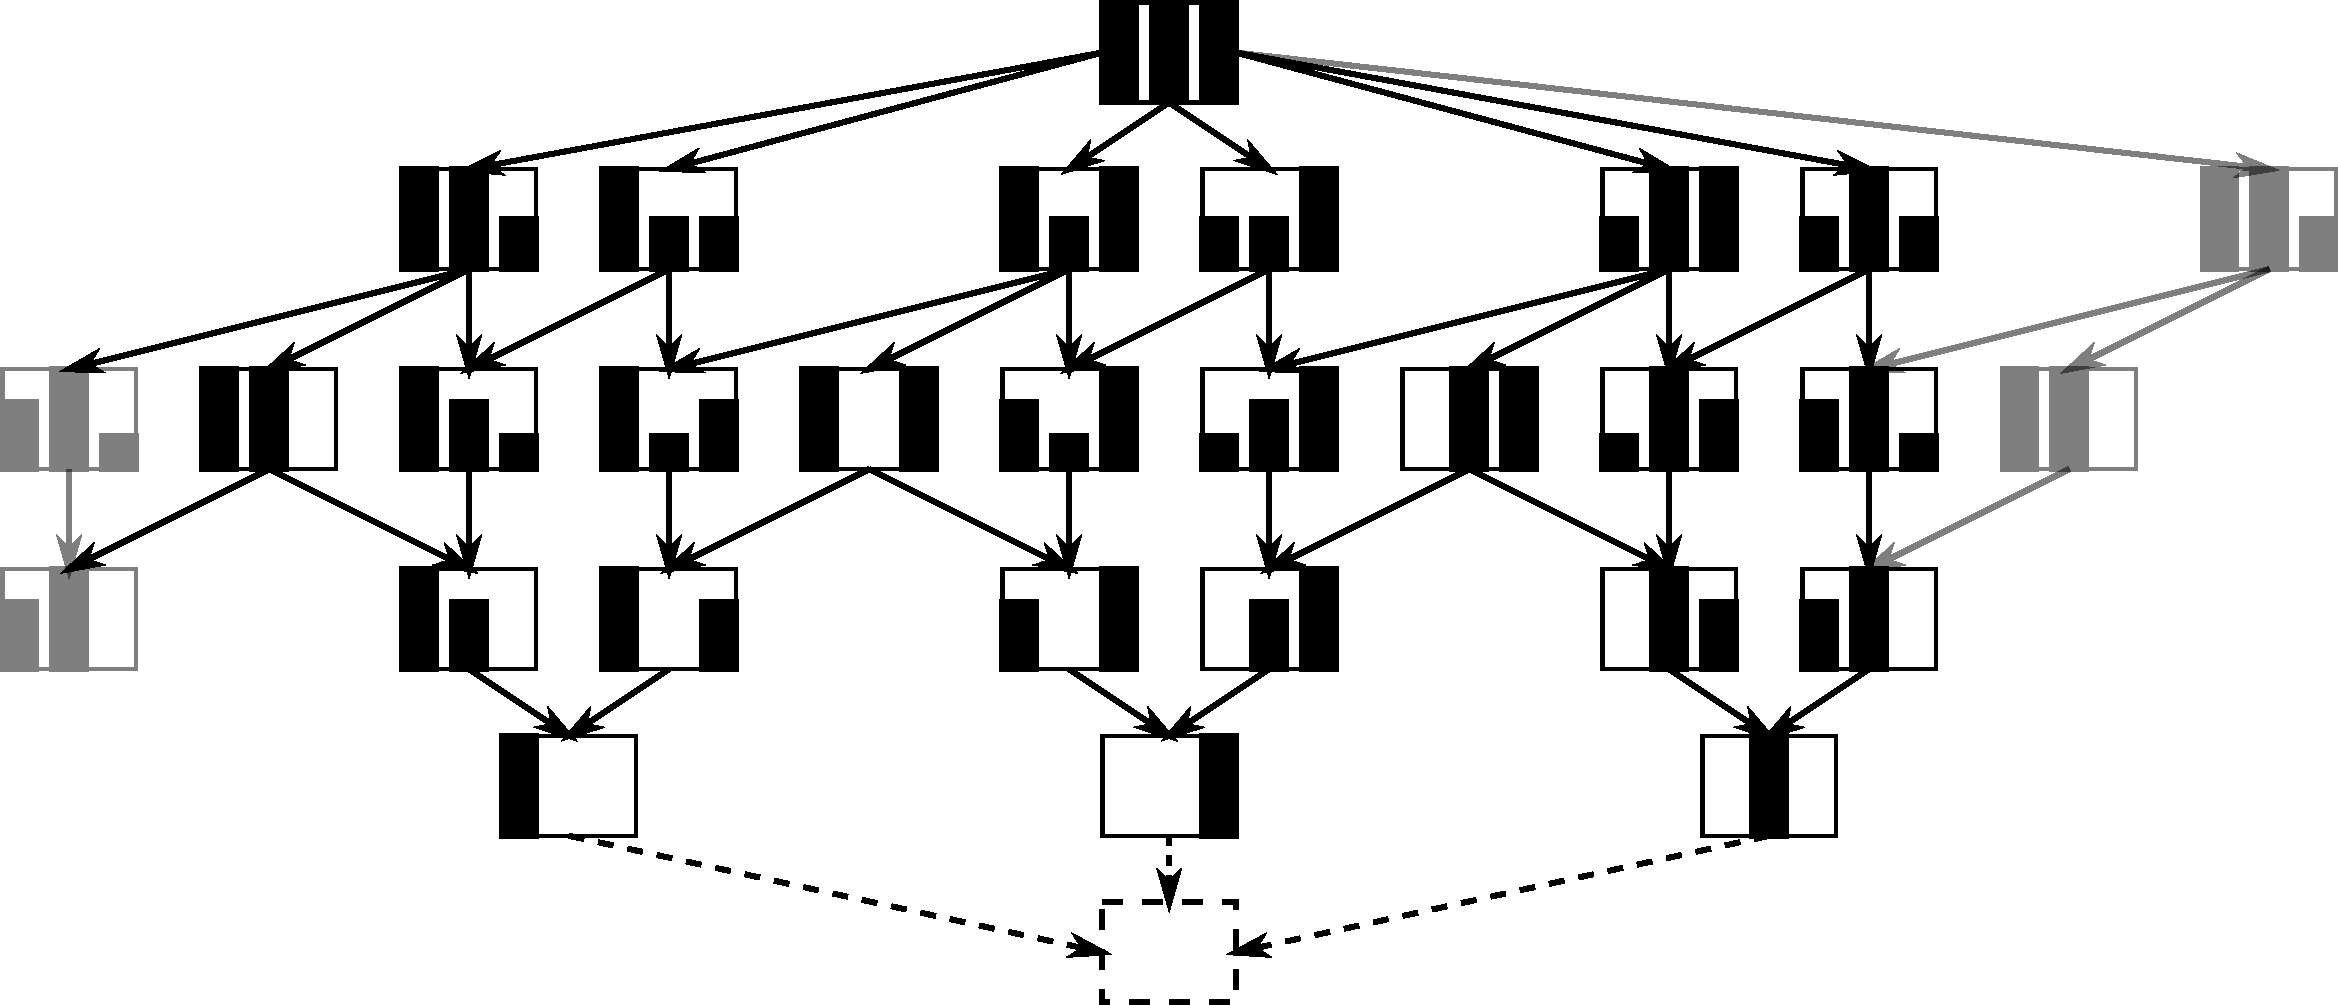
\includegraphics[width=374, height=161, scale=5]{pictures/three-point-omega.pdf}}
\caption{Черные столбчатые диаграммы представляют все неэквивалентные распределения возможностей в случае $\Omega = \{\omega_1, \omega_2, \omega_3 \}$, $i$-ый столбей каждой диаграммы --- $\pi(\omega_i)$ в высоту. Любое другое распределение эквивалентно одному из распределений, показанных на рисунке. Стрелки демонстрируют отношение специфичности ``$\preceq$''. Они указывают от менее специфичных распределений к более специфичным. Столбчатые диаграммы, показанные серым цветом, являются дубликатами черных столбчатых диаграмм, они добавлены к рисунку, чтобы избежать стрелок, пересекающих его слева направо и наоборот. Пунктирный прямоугольник соответствует квазираспределению $\textbf{0}(\cdot) = 0$.}
\end{figure}

Квартет $(\widetilde{\varpi}, \preceq, \lor, \land)$, состоящий из расширенного множества $\widetilde{\varpi}$ распределений возможностей, отношения специфичности ``$\preceq$'' на $\widetilde{\varpi}$, операций ``$\lor$'' и ``$\land$'' на $\widetilde{\varpi}$ --- является \textbf{решеткой}. Действительно, $\textbf{0} \preceq \pi \preceq \textbf{1}$ для любого $\pi \in \widetilde{\varpi}$, где $\textbf{1} \in \widetilde{\varpi}$ определеяется, как $\textbf{1}(\omega) = 1$ для любого $\omega \in \Omega$. Супремум $\pi_1 \lor \pi_2$ и инфимум $\pi_1 \land \pi_2$ определены для всех $\pi_1, \pi_2 \in \widetilde{\varpi}$ (см. \cite{ag-op-2021}). 

Решетка $(\widetilde{\varpi}, \preceq, \lor, \land)$ может быть использована в качестве основы для алгебры субъективных суждений, выраженных через распределения возможностей. Эта алгебра может быть использована при групповом принятии решений для достижения “положительного” и “отрицательного” консенсуса между экспертами, как описано выше.

\section{Алгоритм нахождения расстояния между распределениями возможностей и мера специфичности}

\subsection{Описание алгоритма нахождения расстояния между распределениями возможностей}

Будем рассматривать решетку на классах эквивалентностей как ориентированный граф, в котором вершины являются распределениями возможностей из $\widetilde{\varpi}$, а дуги ориентированы от менее специфичных распределений к более специфичным. Пусть есть два распределения $\pi_1$ и $\pi_2 \in \widetilde{\varpi}$, $\pi_2 \preceq \pi_1$. В теории графов расстоянием между двумя вершинами графа называется число дуг в кратчайшем пути. Задача заключается в нахождении расстояния между $\pi_1$ и $\pi_2$.\\

\textbf{Первый шаг алгоритма. Перестановка событий в $\Omega = \{ \omega_1, \omega_2, \ldots, \omega_n \}$.} Переупорядочим события так, чтобы их возможности и в первом и во втором распределении были упорядочены по невозрастанию:
\begin{equation}
    1\rightarrow i_1, 2 \rightarrow i_2, \ldots, n \rightarrow i_n
\end{equation}
\begin{figure}[h!]
\center{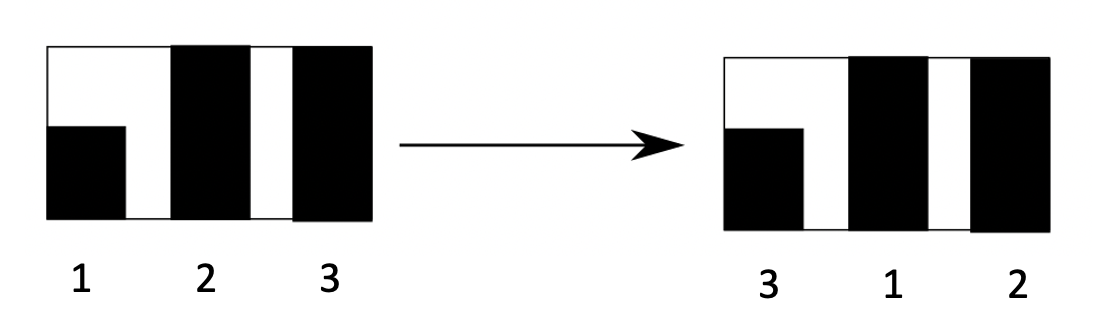
\includegraphics[width=210, height=70, scale=5]{pictures/image_11.png}}
\caption{Перестановка событий}
\end{figure}

\textbf{Второй шаг алгоритма. Ставим каждому из распределений в соответствие число $e$.} В теории возможностей \cite{pytev-poss-textbook-main} вводиться двоичное число $e \in (0,1)$, $e=0,e_1e_2\ldots e_n$,
которое определялось следующим образом:
\begin{equation}
    e_i =
      \begin{cases}
        1,    & \quad \text{если} \quad \pi(\omega_i) > \pi(\omega_{i+1})\\
        0,  & \quad \text{если } \quad \pi(\omega_i) = \pi(\omega_{i+1})
      \end{cases},\quad i = \overline{1, n-1}
\end{equation}
Расширим данное определение. Будем записывать в числе $e$ не только упорядоченности возможностей, но также, для наименьшей возможности, больше она или равна нулю. Это пригодится нам в дальнейшем.
\begin{equation}
    e_n =
      \begin{cases}
        1,    & \quad \text{если} \quad \pi(\omega_n) > 0\\
        0,  & \quad \text{если } \quad \pi(\omega_n) = 0
      \end{cases}
\end{equation}
Поставим распределениям $\pi_1$ и $\pi_2$ в соответствия числа $e_1$ и $e_2$:
$$\pi_1 \rightarrow e_{\pi_1},$$
$$\pi_2 \rightarrow e_{\pi_2}.$$

\textbf{Несколько замечаний перед переходом к третьему шагу алгоритма.}
\begin{definition}
Сюръекция, или сюръективное отображение --- отображение множества X на множество Y $f: X \to Y$, при котором каждый элемент множества Y является образом хотя бы одного элемента множества X, то есть $\forall y \in Y \quad \exists x \in X : y = f(x)$.
\end{definition}
\begin{figure}[h!]
\center{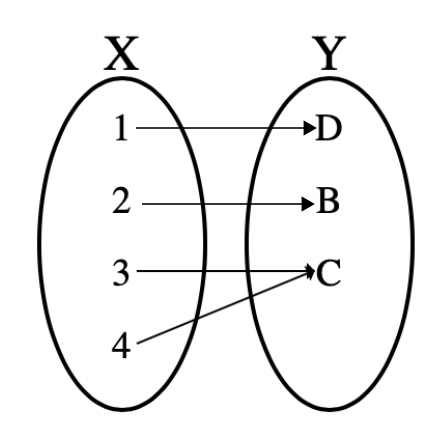
\includegraphics[width=130, height=125, scale=5]{pictures/surection.png}}
\caption{Сюръективное отображение}
\end{figure}
\begin{definition}
Два графа называются изоморфными, если у
них одинаковое число вершин (обозначим его n) и вершины каждого из них можно
занумеровать так числами от 1 до n, что в первом графе две вершины соединены дугой
тогда и только тогда, когда вершины с такими же номерами во втором графе соединены, и ориентации дуг в обоих графах совпадают.
\end{definition}

Множество качественных распределений возможностей можно сюръективно отобразить на множество двоичных чисел $e$. При таком отображении каждый элемент из множества двоичных чисел $e$ будет изображением как минимум одного распределения из множества качественных распределений возможностей. При этом подграфы графа качественных распределений возможностей будут изоморфны графу двоичных чисел $e$, а их объединение представляет собой полный граф. Из изоморфности подграфов графу двоичных чисел $e$ следует, что можно искать расстояние между $\pi_1$ и $\pi_2$ в графе качественных распределений как расстояние между числами $e_{\pi_1}$ и $e_{\pi_2}$ в графе двоичных чисел $e$.
\begin{figure}[h!]
\center{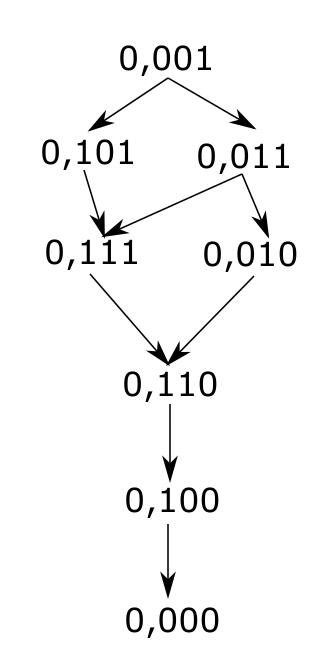
\includegraphics[width=112, height=224, scale=5]{pictures/image_22b.png}}
\caption{Граф двоичных чисел e}
\end{figure}

\textbf{Третий шаг алгоритма. Построение графа двоичных чисел e.} Для нахождения расстояния между $e_{\pi_1}$ и $e_{\pi_2}$ не требуется строить граф целиком. Нужна толька та его часть, которая лежит между $e_{\pi_1}$ и $e_{\pi_2}$. Обход начинается от вершины, которая соответствует менее специфичному распределению, и заканчивается, когда доходит до вершины, которая соответствует более специфичному.

Каждый переход представляет собой изменение одного знака в упорядоченности возможностей: знак больше меняется на знак равно или наоборот, то есть, если рассматривать с точки зрения двоичного числа $e$ у нас меняется одна цифра после запятой: нуль на единицу или единица на нуль.

Рассмотрим граничные случаи:
\begin{enumerate} 
    \item Нули, которые стоят в конце числа e, не меняются $e=0,010\ldots1{\color{red}0\ldots0}$, так как это означает, что соответствующие возможности уже равны нулю, и их нельзя повысить, так как тогда нарушится отношение специфичности.
    \begin{figure}[h!]
    \center{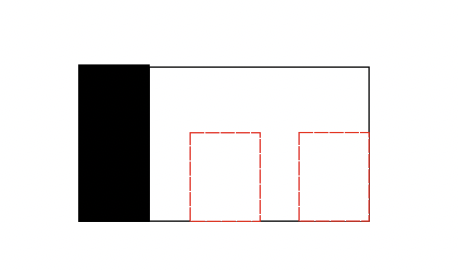
\includegraphics[width=90, height=45, scale=5]{pictures/image_2.png}}
    \caption{Нули, которые стоят в конце числа e не меняются}
    \end{figure}
    \item Также особого рассмотрения заслуживает случай, когда все цифры в числе $e$  равны нулю, кроме последней $e=0,00{\color{red}0\ldots01}$. Такое число $e$ соответствует наименее специфичному распределению возможностей: $\pi(\omega_1)=\pi(\omega_2)=\ldots=\pi(\omega_n)>0$. Соответственно, можно менять в числе $e$ нули на единицы, но нельзя поменять последнюю единицу на ноль, так как тогда мы перейдем к распределению $\pi(\omega_1)=\pi(\omega_2)=\ldots=\pi(\omega_n)=0$, то есть к наиболее специфичному распределению, а такого перехода быть не может. Следовательно, для того, чтобы поменять последнюю единицу на ноль, надо, чтобы в $e$ была хотя бы одна единица кроме последней $e=0,00{\color{red}0\ldots010\ldots01}$.
    \begin{figure}[h!]
    \center{
\includegraphics[width=155, height=45, scale=5]{pictures/image_3.png}}
    \caption{Невозможен переход от наименее специфичного распределению к наиболее специфичному}
    \end{figure}
\end{enumerate}

Теперь, ограничив себя этими случаями, рассмотрим какие переходы могут быть сделаны. На каждом шаге есть две опции:
\begin{enumerate}
    \item Поменять последнюю цифру, не равную нулю, на нуль:
    $$e=0,10\ldots1{\color{red}1}0\ldots0\quad\rightarrow\quad e=0,10\ldots1{\color{red}0}0\ldots0$$ Таким образом, самая маленькая, не равная нулю возможность, станет равна нулю.
    \begin{figure}[h!]
    \center{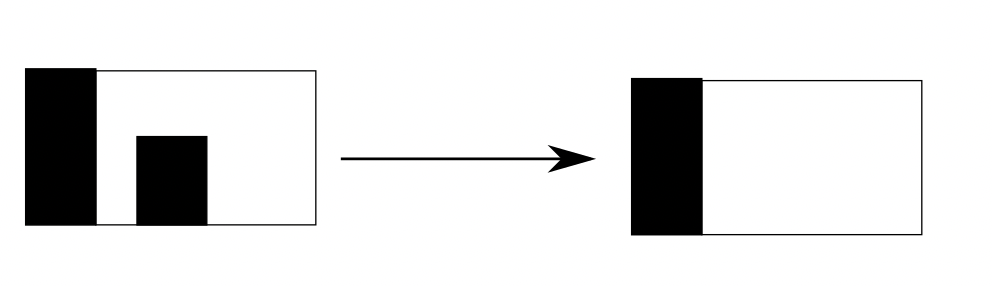
\includegraphics[width=155, height=45, scale=5]{pictures/image_4.png}}
    \end{figure}    
    \item Поменять один из нулей, стоящих до последней единицы в числе e, на единицу.
    $$e=0,1{\color{red}0}0\ldots10\ldots0\quad\rightarrow\quad e=0,1{\color{red}1}0\ldots10\ldots0$$
    Это соответствует переходу: $$\pi(\omega_i)=\pi(\omega_{i+1})\quad\rightarrow\quad\pi(\omega_i)>\pi(\omega_{i+1})$$ Здесь важно отметить, что менять единицу, стоящую до последней, на нуль нельзя, так как это означает, что нам придется увеличить какую-то возможность, которую уже была уменьшена до этого, что нарушит отношение специфичности при переходе.
    \begin{figure}[h!]
    \center{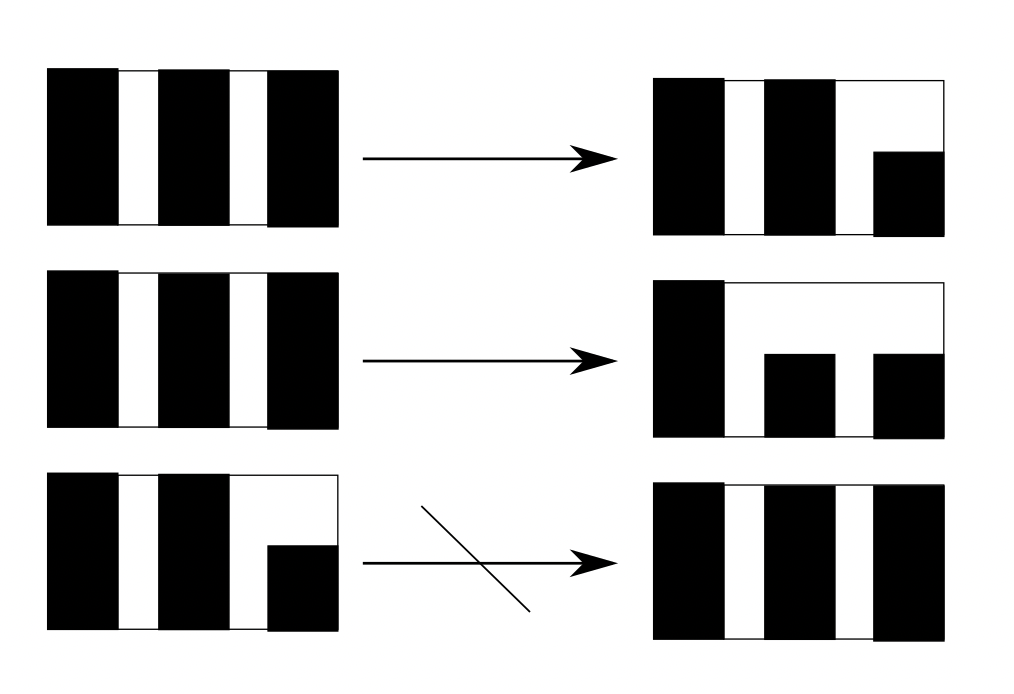
\includegraphics[width=155, height=150, scale=5]{pictures/image_5.png}}
    \end{figure}   
\end{enumerate}

Выше сформулированы правила, по которым делаются переходы в графе двоичных чисел $e$. Перед началом обхода заведем счетчик, равный нулю. С каждым новым переходом будем увеличивать его на единицу. После каждого перехода делаем проверку: совпадает ли текущая вершина с $e_{\pi_2}$. Если совпадает, то это означает, что мы прошли весь путь от $e_{\pi_1}$ до $e_{\pi_2}$, и текущее значение счетчика равно расстоянию между соответствующими вершинами. В таком случае обход заканчивается. Если не совпадает, то значит мы еще не дошли до искомой вершины, и обход продолжается.

\subsection{Возможные реализации алгоритма}
Есть несколько алгоритмов обхода графа. Самые популярные из них, это поиск в глубину (depth-first search --- DFS) и поиск в ширину (breadth-first search --- BFS). Нам подходят оба.

Поиск в глубину --- прямолинейный способ обхода графа. Алгоритм начинает работу в начальной вершине и перебирает все вершины, достижимые из нее по ребрам графа. Поиск в глубину всегда следует по одному пути, пока на нем еще имеются вершины. После этого он возвращается и начинает исследовать другие части графа. Обычно алгоритм запоминает посещенные вершины, так что каждая обходиться только один раз. В нашем случае это также может служить существенной оптимизацией, так как часть путей в графе не приведет нас к искомой вершине, и на каком-то шаге эти пути начнут совпадать. Последней будем считать вершину, в которой распределение совпадает с наиболее специфичным распределением ($e_{cur}=0,0\ldots0$). 

При поиске в ширину вершины графа посещаются в порядке возрастания расстояния от начальной вершины. В процессе обходятся вершины уровень за уровнем. Сначала посещаются вершины, отстоящие от начальной на расстояние 1, затем на расстояние 2 и т.д. Процесс продолжается, пока не останется непосещенных вершин. В нашем случае, алгоритм заканчивает работу, когда мы дошли до $e_{\pi_2}$.

\subsection{Мера специфичности}
Выше описан алгоритм, который позволяет находить расстояние $\rho(\pi_1, \pi_2)$ между двумя распределениями $\pi_1$ и $\pi_2$, $\pi_2 \preceq \pi_1$, в графе качесвенных распределений возможностей. Если рассматривать $\pi_1$ и $\pi_2$ как экспертные оценки событий в $\Omega$, то расстояние между ними может служить мерой специфичности или мерой согласованности между экспертами. Чем меньше расстояние, тем больше согласованы оценки. Если $\pi_1$ и $\pi_2$ совпадают, тогда $\rho(\pi_1, \pi_2) = 0$, и это означает, эксперты пришли к полному консенсусу, их мнения совпали касательно всех $\omega_i \in \Omega$, $i = \overline{1, n}$, и в $\pi_1$ и $\pi_2$ все события упорядочены одинаково. Тогда меру специфичности можно задать, например, как:
\begin{equation}
    \varphi(\pi_1, \pi_2) = \frac{\rho_{max} - \rho(\pi_1, \pi_2)}{\rho_{max}},
\end{equation}
где $\rho_{max} = 2n - 1$, так как расстояние между наименее специфичным и наиболее специфичным распределением равно 2n. Доказывается по индукции добавлением в $\Omega$ $\omega_{n+1}$.

Тогда, $\varphi(\pi_1, \pi_2): \widetilde{\varpi} \times \widetilde{\varpi} \to [0, 1]$, и чем больше $\varphi$ к единице, тем больше согласованы экспертные оценки. Если $\varphi = 0$, значит экспертные оценки полностью рассогласовны.

Особого внимания заслуживает случай, когда $\pi_1$ и $\pi_2$ не сравнимы с помощью отношения специфичности ``$\preceq$''. Тогда невозможно перейти от одного распределения в графе к другому и посчитать расстояние $\rho(\pi_1, \pi_2)$. Чтобы решить эту проблему, в подобных случаях будем сначала находить $\pi_1 \lor \pi_2$ и $\pi_1 \land \pi_2$, а затем считать расстояние между супремумом и инфимумом $\rho(\pi_1 \lor \pi_2, \pi_1 \land \pi_2)$, то есть расстояние между ``позитивным'' и ``негативным'' консенсумами, тогда мера спефичности будет иметь вид:
\begin{equation}
    \varphi(\pi_1, \pi_2) = \frac{\rho_{max} - \rho(\pi_1 \lor \pi_2, \pi_1 \land \pi_2)}{\rho_{max}}.
\end{equation}
В \cite{ag-op-2021} доказывается, что $\pi_1 \lor \pi_2$ и $\pi_1 \land \pi_2$ всегда можно упорядочить с помощью ``$\preceq$''.
\section*{Выводы}
В рамках работы был рассмотрены и изучены различные разделы теории возможностей Ю.П. Пытьева, отношение специфичности ``$\preceq$'', супремум ``$\lor$'' и инфимум  ``$\land$'' и их возможное приложение в принятии решений.

Был разработан, а также реализован алгоритм, который позволяет находить расстояние между различными распределениями в решетке на классах эквивалентностей, а также рассмотрен случай когда распределения не могут быть упорядочены с помощью отношения специфичности ``$\preceq$''.

Распределения возможностей можно рассматривать как экспертные оценки по различным вопросам, рейтинги, топы и т.д. Было предложено возможное определение меры специфичности (меры согласованности), которая показывает на сколько согласованы различные экспертные оценки.


\newpage
\printbibliography[heading=bibintoc]


\end{document}
